\section{Our Structure}

\subsection{Kinect Node: Gestures}

\subsection{Action Node: Katana \& Scout Movement}
\subsubsection{Katana}
As mentioned in section \ref{Material: Katana} with help of the \textit{ROS} package \textit{Katana Native Interface} it is possible to power-off the motors of the robotic arm while keeping the robot communicating with the computer.

While the motors are off, one can move the arm to the desired positions and afterwards read the values of the joint positions. Doing this repeatedly using all the desired positions, it is possible to program movement sequences, creating a gesture. After having each step of the movement, we programmed the maximum time for executing each step of the gesture. As well as for the positions, these maximum times were empirically determined. In the end of each movement, Katana goes to a defined default position.

Using this line of thought we created the following gestures: high-five, low-five, clap, wave, pass the slide and grab.

Since Katana as 7 degrees of freedom (6 joints and the gripper), the structures sent to Katana are a vector with 7 entries.
\begin{center}
General structure:
$\left[ Joint1, Joint2, Joint3, Joint4, Joint5, Joint6, Gripper\right]$\\
\end{center}
Using as an example the gesture "wave", the maximum time for reaching each position and the position goal sequence are given by:
\begin{center}
Maximum time:
$\left[5, 1.3, 1.3, 1.3, 5\right]$\\
\end{center}
\begin{table}[!h]
\centering
\begin{tabular}{lc}
Position 1: & {[}-1.85, 1.57, 0.175, -0.35, -1.57, 0.175, 0.175{]} \\
Position 2: & {[}-1.85, 1.57, 0.175, 0.35, -1.57, 0.175, 0.175{]}  \\
Position 3: & {[}-1.85, 1.57, 0.175, -0.35, -1.57, 0.175, 0.175{]} \\
Position 4: & {[}-1.85, 1.57, 0.175, 0.35, -1.57, 0.175, 0.175{]}  \\
Position 5: & Default Position                                    
\end{tabular}
\caption{Wave Sequence}
\label{wave}
\end{table}

Looking at the table~\ref{wave} we can observe that in this movement the only joint that changes its position is Joint 4, similar to the human gesture where the only joint that moves while waving is the elbow joint.

\subsubsection{Scout}
The Scout robot is a two wheel, two motor differential drive robot, that means that for controlling the robot, one needs a linear and an angular velocity. One can translate these two velocities to the velocities of each wheel, by using following equations:
\begin{equation}
v_{lin} = \frac{(\omega_{right}+\omega_{left})r}{2} \\
\end{equation}
\begin{equation}
v_{ang} = \omega = \frac{(\omega_{right}-\omega_{left})r}{2d}
\end{equation}
Where $r$ represents the radius of the wheel, and $d$ the distance between wheels.
As it can be seen in figure \ref{fig:scout_axis} our robot has two degrees of freedom, but since the movement of the robot isn't the main point of this project, we assume, as a proof of concept, to only move in the \textit{x}-axis (forwards and backwards).

The implemented controller receives as an input a dislocation. The idea of having as input a final position in the world map, is a possible improvement for future work, but requires the robot tracking by the Kinect Node.

\begin{figure}[!h]
    \centering
    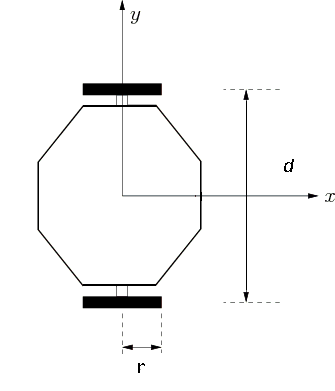
\includegraphics[width=0.5\columnwidth]{./ScoutAxis.png}
    \caption{Scout Axis}
    \label{fig:scout_axis}
\end{figure}
The control loop that we implemented looks as shown in figure \ref{fig:scout_loop}.
\begin{figure}[!h]
    \centering
    \includegraphics[width=\columnwidth]{./ControlLoopScout.png}
    \caption{Scout's Control Loop}
    \label{fig:scout_loop}
\end{figure}

\subsection{Decision Node: Probabilistic Model}
